\chapter{Résumé détaillé}
La résonance magnétique est une technique spectroscopique qui exploite le couplage entre des spins et un rayonnement électromagnétique afin de sonder les propriétés microscopiques de la matière. Ce domaine se divise généralement en résonance paramagnétique électronique (Electron Paramagnetic Resonance, EPR)~\sidecite{abragam_principles_1986} et en résonance magnétique nucléaire (Nuclear Magnetic Resonance, NMR)~\sidecite{slichter_principles_1996}, selon la nature des spins étudiés : respectivement des spins électroniques célibataires (électrons non appariés) ou des spins nucléaires. En raison de l'omniprésence des spins dans la matière, les techniques de résonance magnétique trouvent de nombreuses applications, allant de l'imagerie médicale~\sidecite{lauterbur_image_1973} à la science des matériaux~\sidecite{haworth_solidstate_2022}, en passant par la biologie~\sidecite{wuthrich_protein_1989} et le contrôle qualité pharmaceutique~\sidecite{holzgrabe_quantitative_2010}.

Une limitation importante des techniques conventionnelles de résonance magnétique est leur faible sensibilité. Comme l'interaction entre les spins et les champs électromagnétiques est faible, de grands ensembles de spins sont nécessaires pour produire un signal détectable. Par conséquent, la plupart des mesures donnent accès à des grandeurs moyennées sur l'ensemble, tandis que les variations microscopiques et locales restent difficiles à atteindre.

En utilisant des amplificateurs limités par le bruit quantique et des résonateurs supraconducteurs, la sensibilité a été poussée à l'extrême, au point de permettre la détection de dix spins électroniques~\sidecite{ranjan_electron_2020}. La détection d'un spin unique a été réalisée dans un petit nombre de systèmes à l'état solide, tels que les centres NV dans le diamant~\sidecite{jelezko_single_2002} et les impuretés donneuses dans le silicium~\sidecite{morello_singleshot_2010}. Cela a été rendu possible grâce à des mécanismes spécifiques à chaque système, notamment des transitions optiques sélectives en spin et la conversion spin-charge. Les résultats obtenus dans ces systèmes montrent comment des spins électroniques et nucléaires individuels dans l'état solide peuvent être utilisés pour le calcul quantique~\sidecite{bradley_tenqubit_2019,edlbauer_11qubit_2025} et la spectroscopie de haute précision~\sidecite{abobeih_atomicscale_2019,breitweiser_quadrupolar_2024}.

Récemment, notre groupe a montré que des impuretés paramagnétiques individuelles dans un diélectrique pouvaient être détectées via la fluorescence micro-onde de leur transition de spin électronique à 10~mK~\sidecite{wang_singleelectron_2023}. Cette méthode est, en principe, applicable à un grand nombre d'espèces paramagnétiques et de substrats, puisqu'elle requiert uniquement d'augmenter le taux d'émission spontanée du spin électronique au-delà du taux de relaxation non radiative à des températures cryogéniques. \textbf{Cette thèse montre comment le comptage de photons micro-ondes peut être utilisé pour détecter et contrôler de manière cohérente des spins nucléaires individuels couplés à un seul spin électronique.} De plus, nous démontrons une spectroscopie de précision des transitions NMR et montrons comment les spins nucléaires peuvent trouver des applications en calcul quantique.

La thèse est divisée en trois parties. La première partie du manuscrit décrit le système physique et le dispositif expérimental. Nous introduisons l'Hamiltonien de spin des spins électroniques de \Er dans \Ca, les spins nucléaires présents dans le cristal et leur interaction. Nous décrivons comment le couplage du spin de \Er à un résonateur accroît le taux de relaxation spontanée via l'effet Purcell, ainsi que le dispositif de détection : le détecteur de photons micro-ondes uniques. En outre, nous présentons les techniques micro-ondes utilisées pour contrôler l'état de spin nucléaire. La deuxième partie de ce travail est consacrée à la détection et au contrôle des spins nucléaires de \W. Nous mesurons des sauts quantiques de l'état de spin nucléaire et démontrons la spectroscopie hyperfine ainsi qu'une préparation déterministe à l'aide de seules impulsions micro-ondes. Par ailleurs, nous utilisons une excitation Raman stimulée par micro-ondes afin de démontrer des portes à un et deux qubits dans un registre à deux qubits de spins nucléaires de \W. Nous mesurons également des temps de cohérence de l'ordre d'une seconde, parmi les plus longs mesurés dans l'état solide. Dans la troisième partie de la thèse, nous étudions une impureté \Nb de spin nucléaire 9/2. Nous généralisons les techniques présentées ci-dessus et réalisons une spectroscopie de précision des transitions de spin nucléaire.

\section*{Mesurer la fluorescence de spins électroniques individuels}
\begin{figure*}[b!]
    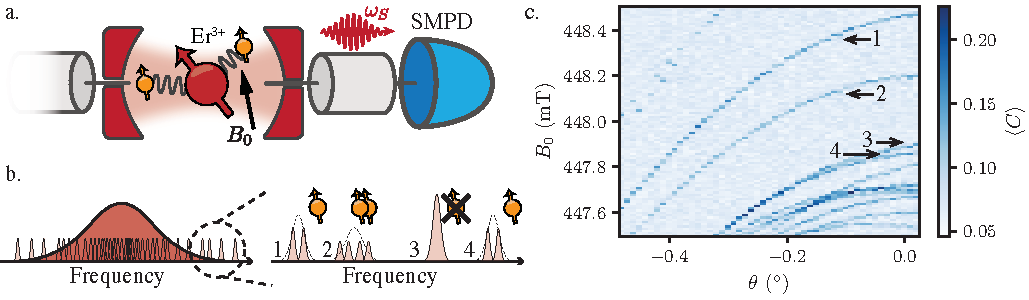
\includegraphics{chapter1/figures/principle.pdf}
    \caption[Principe de mesure]{Dispositif expérimental et principe de mesure.
    \textbf{a.} Le système physique est constitué de spins électroniques individuels (rouge) couplés magnétiquement à leur environnement de spins nucléaires (orange) ainsi qu'à une cavité supraconductrice. Le spin électronique (de fréquence $\omega_S$) est porté dans son état excité par une impulsion micro-onde (gaussienne, rouge). Le taux de relaxation spontanée est augmenté par l'effet Purcell, et la fluorescence micro-onde (ligne rouge) est collectée par un détecteur de photons micro-ondes uniques (SMPD).
    \textbf{b.} Élargissement inhomogène et élargissement dipolaire nucléaire. \textit{(gauche)} Le rapport gyromagnétique de chaque spin \Er est modifié par l'environnement local, et le signal d'ensemble est donc élargi. Cet effet, appelé élargissement inhomogène, est présent à l'état solide en raison des contraintes locales et des mécanismes de compensation de charge à la position de chaque ion. \textit{(droite)} Sur les ailes du signal élargi inhomogènement, des spins individuels peuvent être résolus. À l'échelle du spin unique, la fréquence de résonance dépend du bain de spins nucléaires, auquel le spin électronique est couplé par interaction dipolaire magnétique. Si le couplage entre spins électroniques et nucléaires est plus fort que le taux de décohérence du spin électronique, plusieurs pics peuvent être résolus.
    \textbf{c.} Spectroscopie par comptage de photons en fonction de l'amplitude et de l'angle du champ magnétique. L'augmentation du nombre moyen de comptages détectés $\langle C \rangle$ correspond au signal de fluorescence d'un ou plusieurs spins. Des spins individuels peuvent être résolus, et les différences de rapport gyromagnétique dues à l'élargissement inhomogène apparaissent clairement.
    }
    \labfig{principle}
\end{figure*}

Les spectromètres EPR impulsionnels conventionnels mesurent la magnétisation transverse d'ensembles de spins électroniques, qui rayonnent collectivement un champ cohérent détecté par une antenne proche. Les efforts visant à accroître la sensibilité de la spectroscopie EPR pour la détection de petits échantillons ont conduit à concevoir des résonateurs de détection à faible volume de mode, ce qui est avantageusement obtenu à l'aide de résonateurs métalliques plans. Des électrodes en métal normal conduisent à des facteurs de qualité dans la gamme 10--100~\sidecite{narkowicz_scaling_2008,dayan_advanced_2018}, tandis que des facteurs de qualité plus élevés et des volumes de mode plus faibles peuvent être atteints avec des résonateurs supraconducteurs~\sidecite{wallace_microstrip_1991}. Notre groupe a poussé ces efforts à la limite en refroidissant l'échantillon à des températures millikelvin et en utilisant des amplificateurs micro-ondes supraconducteurs atteignant la limite quantique de sensibilité~\sidecite{bienfait_reaching_2016}, obtenant une sensibilité suffisante pour détecter 10 spins avec un temps d'intégration d'une seconde~\sidecite{ranjan_electron_2020}. In fine, le bruit résiduel est entièrement dû aux fluctuations du vide du champ micro-onde. Bien que ces dernières puissent être légèrement réduites au moyen d'états micro-ondes comprimés (squeezed)~\sidecite{bienfait_magnetic_2017}, cela n'a pas suffi pour atteindre la sensibilité au spin unique.

Une nouvelle méthode de détection pour la spectroscopie EPR, permettant de dépasser ces limitations, a été récemment démontrée dans notre groupe, comme illustré sur la \reffig{principle}a. Cette méthode repose sur la détection de la fluorescence micro-onde émise par les spins électroniques lorsqu'ils relaxent vers leur état fondamental, de façon analogue aux techniques de comptage de photons dans le domaine optique~\sidecite{albertinale_detecting_2021}. Pour mesurer cette fluorescence, nous utilisons un détecteur de photons micro-ondes uniques (Single Microwave Photon Detector, SMPD), un dispositif supraconducteur qui associe l'arrivée d'un photon à l'état d'un qubit transmon~\sidecite{lescanne_irreversible_2020}. En détectant l'énergie du photon plutôt que sa quadrature, la technique est insensible aux fluctuations du vide. Toutefois, la détection de spins électroniques via leur fluorescence micro-onde doit surmonter un obstacle majeur : le taux d'émission spontanée d'un spin dans l'espace libre est extrêmement faible ($10^{-12}~\mathrm{s}^{-1}$) et, à l'état solide, la décroissance non radiative via l'interaction avec les phonons constitue le mécanisme dominant.

En couplant inductivement les spins électroniques à un résonateur de faible volume de mode et de fort facteur de qualité, le taux de relaxation radiative peut être amplifié via l'effet Purcell~\sidecite{purcell_spontaneous_1946}. Des résonateurs supraconducteurs ont permis de démontrer des facteurs de Purcell de l'ordre de $10^{14}$, conduisant à des taux de relaxation radiative de l'ordre de $10^{3}~\mathrm{s}^{-1}$. Cette augmentation extrême est rendue possible par la nature supraconductrice des dispositifs, qui réduit fortement les pertes internes, et par la concentration du champ magnétique dans une petite région au moyen d'éléments inductifs localisés tels que des nanofils~\sidecite{wang_singleelectron_2023}.

Par ailleurs, deux difficultés peuvent être atténuées lorsqu'on opère à des températures cryogéniques. Premièrement, le rayonnement micro-onde du corps noir est exponentiellement supprimé, ce qui réduit le nombre de photons thermiques à l'entrée du SMPD et améliore ainsi le rapport signal-sur-bruit de détection. Deuxièmement, le bain de phonons est « gelé » et le taux de relaxation non radiative est réduit. Dans ces conditions, il a été possible de démontrer la détection d'un spin unique par comptage de photons micro-ondes~\sidecite{wang_addressing_2023, balembois_magnetic_2023, pallegoix_high_2025}.

\begin{marginfigure}
    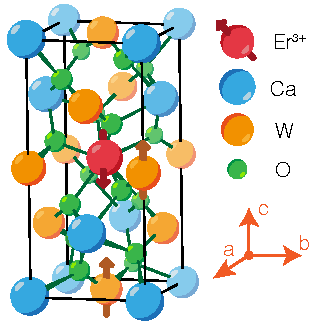
\includegraphics{chapter2/figures/crystal.pdf}
    \caption[Cristal \Ca]{Première maille élémentaire d'un cristal de \Ca, centrée autour d'un ion \Er substitutionnel.}
    \labfig{crystal_structure_ch1}
\end{marginfigure}

Le schéma de mesure est représenté sur la \reffig{principle}a. Un spin électronique est couplé à une cavité résonante (tous deux en rouge). La cavité est couplée à deux ports, entrée et sortie. Une excitation micro-onde (gaussienne, rouge) porte le spin électronique dans l'état excité. Le spin relaxe rapidement via l'effet Purcell et émet un photon incohérent dans le port de sortie, lequel est acheminé vers le SMPD où il est détecté. Le spin électronique est également couplé aux spins nucléaires de l'environnement (orange) via l'interaction hyperfine. L'état du spin nucléaire influence donc la fréquence du spin électronique, et la résolution de ces décalages permettrait la détection d'un spin nucléaire unique.

Les spins électroniques dans les solides possèdent des fréquences de Larmor différentes en raison de variations de leur environnement local électrostatique ou magnétique. Il en résulte que la largeur spectrale du signal d'ensemble est beaucoup plus grande que la largeur des composantes associées à chaque spin individuel (voir \reffig{principle}b). Cet « élargissement inhomogène » limite la résolution spectrale en spectroscopie EPR et constitue l'une des motivations de l'EPR à spin unique. Dans les expériences présentées dans cette thèse, l'élargissement inhomogène nous aide au contraire à adresser des spins individuels situés sur les bords de la distribution inhomogène, comme illustré sur la \reffig{principle}b.

Pour réaliser nos expériences, nous utilisons le degré de liberté de spin d'un ion \Er dans \Ca. La première maille élémentaire du cristal est représentée sur la \reffig{crystal_structure_ch1}, l'ion \Er étant au centre. Ces ions sont des impuretés paramagnétiques dans le réseau cristallin, possédant un spin électronique non apparié. Ils peuvent être décrits efficacement comme un spin électronique $S=1/2$ de fréquence $\omega_S$ avec un facteur gyromagnétique anisotrope. Le matériau hôte est choisi en raison de sa faible densité de moments magnétiques nucléaires, ce qui permet d'obtenir de longs temps de cohérence pour le spin électronique~\sidecite{ledantec_twentythreemillisecond_2021}. Un motif de rotation résolu au niveau du spin unique est présenté sur la \reffig{principle}c. La figure montre le nombre moyen de comptages mesuré $\langle C \rangle$ après excitation micro-onde en fonction de l'amplitude et de l'angle du champ magnétique. Une augmentation de $\langle C \rangle$ indique la présence d'un ou plusieurs spins \Er. Chaque parabole correspond à un spin \Er unique avec un facteur gyromagnétique différent et peut être suivie indépendamment en fonction de $\theta$. Dans ce manuscrit, nous étudions l'environnement de spins nucléaires de ces spins et sondons leurs interactions avec les spins nucléaires voisins.

\section*{Détection de spins nucléaires individuels et polarisation nucléaire dynamique}
\begin{figure*}[b!]
    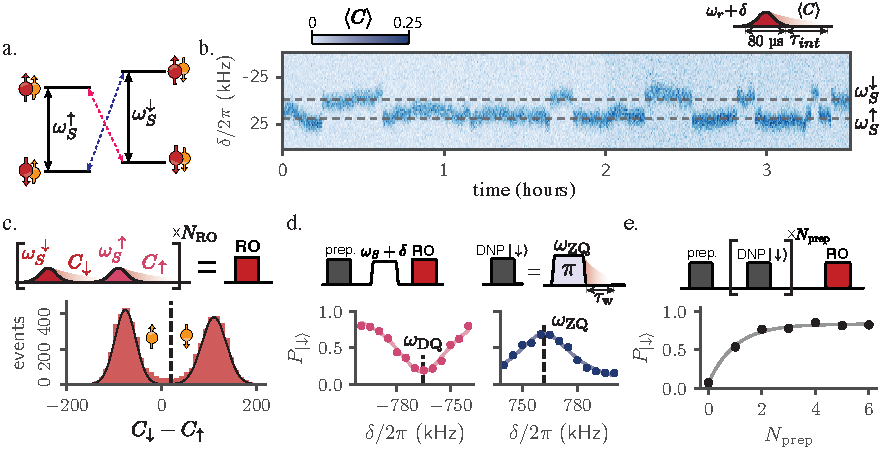
\includegraphics{chapter1/figures/ch1.pdf}
    \caption[Détection de spins individuels de \W et DNP]{
        Détection de spins nucléaires individuels et polarisation nucléaire dynamique.
        \textbf{a.} Système de niveaux d'énergie d'un spin électronique \Er couplé à un spin nucléaire \W. Les états associés aux niveaux d'énergie sont représentés schématiquement. Les deux transitions EPR permises sont indiquées par des flèches noires, et les transitions ZQ et DQ par des flèches pointillées bleues et rouges.
        \textbf{b.} Spectroscopie par comptage de photons d'un spin \Er unique en fonction du temps. Le spin \Er est accordé sur la fréquence du résonateur et une impulsion micro-onde à la fréquence $\omega_r+\delta$ est appliquée à l'échantillon, suivie d'une intégration des comptages avec le SMPD. Les comptages moyennés sur l'ensemble $\langle C \rangle$ sont tracés en fonction de la fréquence de l'impulsion et du temps de mesure. Les deux fréquences EPR permises sont mises en évidence par une ligne grise pointillée. La séquence d'impulsions est indiquée en bas à droite.
        \textbf{c.} Lecture en un seul coup (single-shot) de l'état du spin nucléaire. \textit{(haut)} Séquence d'impulsions de lecture. Le nombre de comptages après excitation de chacune des transitions EPR permises est mesuré pendant $N_\text{RO}$ itérations afin d'obtenir $C_\downarrow$ et $C_\uparrow$. \textit{(bas)} Distribution de $C_\downarrow - C_\uparrow$ pour $N_\text{RO}=10^3$ avec événements. La ligne verticale pointillée fixe le seuil de lecture de l'état nucléaire.
        \textbf{d.} Spectroscopie EDNMR sur spin unique. \textit{(haut gauche)} Séquence d'impulsions EDNMR. Après préparation du spin nucléaire dans $\ket{\downarrow}$ ou $\ket{\uparrow}$, une impulsion de fréquence $\omega_S + \delta$ est appliquée à l'échantillon, suivie d'une lecture nucléaire. \textit{(haut droite)} Définition de l'impulsion de DNP. Une impulsion $\pi$ est appliquée à la fréquence de la bande latérale ZQ, suivie d'un temps d'attente $\tau_\text{w}=5~$ms. \textit{(bas)} Population du spin nucléaire en fonction de la fréquence $\delta$ de l'impulsion EDNMR. Le spin nucléaire a été préparé dans $\ket{\downarrow}$ ($\ket{\uparrow}$) pour le graphe de gauche (droite).
        \textbf{e.} DNP sur spin unique. \textit{(haut)} Séquence d'impulsions. Le spin est préparé dans l'état $\ket{\uparrow}$, puis $N_\text{prep}$ impulsions de DNP sont appliquées, avant la lecture nucléaire. \textit{(bas)} Population du spin nucléaire en fonction du nombre d'impulsions de DNP $N_\text{prep}$. Les données (marqueurs) sont ajustées par une courbe exponentielle (ligne).
    }
    \labfig{ch1}
\end{figure*}

Dans la deuxième partie du manuscrit, nous présentons les principaux résultats expérimentaux obtenus dans cette thèse. Dans le Chapitre \ref{ch:detection_and_control_of_individual_w}, nous démontrons des méthodes permettant de lire l'état, de mesurer le spectre et de polariser des spins nucléaires à proximité immédiate des spins électroniques. Nous tirons parti de la sensibilité au spin électronique unique et de la longue cohérence des spins \Er pour détecter des spins nucléaires proches. Le bain nucléaire dans \Ca est dominé par les spins nucléaires \W, avec une abondance d'environ $\sim14$\%. Par conséquent, chaque spin \Er peut avoir un environnement différent : certains n'auront aucun \W voisin\sidenote{Nous utilisons « voisin » pour désigner des sites du réseau situés dans la première maille élémentaire du cristal, centrée autour de l'impureté.}, tandis que d'autres pourront en avoir plusieurs. Comme illustré sur la \reffig{ch1}a, lorsqu'un spin \Er est couplé à un spin nucléaire \W, le couplage hyperfin scinde les fréquences de transition du spin électronique selon l'état du spin nucléaire \W, $\omega_S^\uparrow$ et $\omega_S^\downarrow$.

Dans le Chapitre \ref{ch:detection_and_control_of_individual_w}, nous sondons l'environnement de spins nucléaires par spectroscopie EPR à haute résolution, à champ magnétique fixé, dans une configuration où un \Er unique est en résonance avec la cavité. Nous mesurons le nombre de comptages après une impulsion micro-onde en fonction de la fréquence de l'impulsion et du temps (voir \reffig{ch1}b). Pour certains spins \Er, la fréquence présente un comportement télégraphique, que nous associons à des sauts quantiques, en temps réel, de l'état d'un spin nucléaire \W voisin.

En exploitant la séparation spectrale des transitions du spin électronique, nous obtenons une lecture en un seul coup, sans démolition quantique (QND), de l'état du spin nucléaire. Le protocole de lecture applique deux impulsions micro-ondes entrelacées, chacune à l'une des transitions EPR permises, et collecte les comptages de fluorescence après chaque impulsion. L'histogramme de la différence de comptages montre deux pics symétriques et nettement résolus (voir \reffig{ch1}c), ce qui permet une lecture single-shot de l'état du spin nucléaire.

Les transitions zéro-quantum et double-quantum (représentées sur la \reffig{ch1}a par des flèches pointillées) sont faiblement permises en raison du terme anisotrope de l'interaction hyperfine et changent simultanément l'état du spin électronique et du spin nucléaire. En EPR d'ensemble, ces transitions faiblement permises sont exploitées dans des mesures d'ELDOR-detected NMR (EDNMR) pour sonder les spectres hyperfins~\sidecite{schosseler_pulsed_1994}. Ici, nous démontrons une EDNMR sur spin unique en excitant les transitions ZQ/DQ sur un spin \Er unique. Nous utilisons les spectres obtenus (montrés sur la \reffig{ch1}d) pour identifier le spin nucléaire couplé comme étant un \W.

\begin{figure*}[b!]
    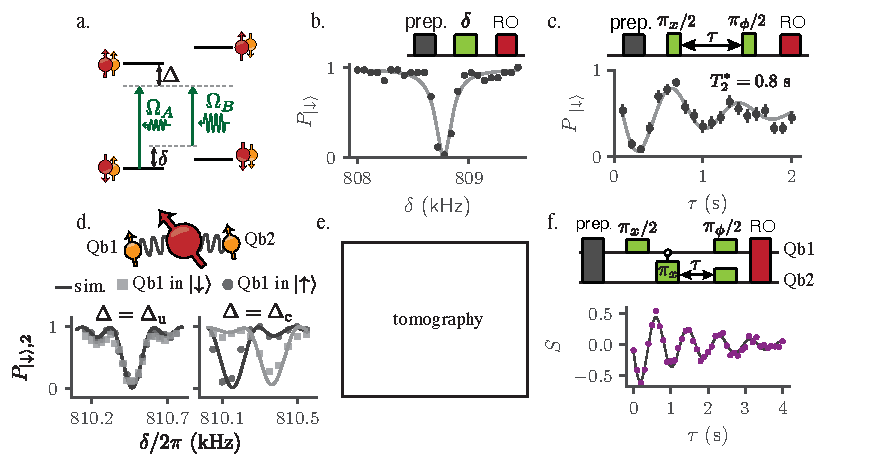
\includegraphics{chapter1/figures/ch2.pdf}
    \caption[Registre de qubits à deux spins nucléaires]{Registre de qubits à deux spins nucléaires.
    \textbf{a.} Schéma Raman stimulé micro-onde dans le système de spins \Er--\W. Les deux impulsions micro-ondes ont des amplitudes $\Omega_\text{A, B}$ et la différence de fréquence entre les deux impulsions est définie comme $\delta$. $\Delta$ est le désaccord (detuning) entre l'excitation A et la transition du spin électronique lorsque le spin nucléaire est dans $\ket{\uparrow}$.
    \textbf{b.} Spectroscopie Raman stimulée. Spectroscopie d'un spin nucléaire \W à l'aide d'impulsions Raman stimulées avec un désaccord $\Delta / 2\pi = -404.8$~kHz. Les lignes continues sont des ajustements lorentziens.
    \textbf{c.} Mesure de Ramsey d'un spin nucléaire \W individuel. L'ajustement (ligne continue) donne $T_2^*=0.8(2)$~s et les barres d'erreur indiquent l'erreur standard sur la moyenne. La phase de la dernière impulsion est $\phi= \omega^\text{art} \cdot \tau$, où $\omega^\text{art}$ est un désaccord artificiel. La différence entre la fréquence du spin nucléaire et le désaccord artificiel est à l'origine des oscillations observées dans les données.
    \textbf{d.} Mise en œuvre d'une porte à deux qubits. \textit{(haut)} Schéma du système mesuré. Un spin \Er unique est couplé simultanément à deux spins nucléaires \W, qui forment le registre quantique : Qb1 et Qb2. \textit{(bas)} Spectroscopie de Qb2 en fonction de l'état de Qb1. Dans le graphe de gauche (droite), les impulsions Raman sont appliquées dans le régime inconditionnel (conditionnel). La ligne continue correspond à une simulation d'évolution temporelle hamiltonienne réalisée avec le logiciel \texttt{QuTiP}.
    \textbf{e.} Tomographie d'un état de Bell. Représentation « city plot » des matrices de densité reconstruites par tomographie de l'état de Bell $\ket{\Psi^+}=\tfrac{1}{\sqrt2}\left(\ket{\downarrow\uparrow}+\ket{\uparrow\downarrow}\right)$. La fidélité extraite après correction des erreurs SPAM est de 0{,}79.
    \textbf{f.} Sous-espace sans décohérence. Mesure de cohérence de Ramsey de l'état $\ket{\Psi^+}$. Un ajustement cosinus amorti exponentiellement donne $T_2^*=1.7(2)~$s. Les deux dernières impulsions $\pi/2$ portent une phase $\phi$ jouant le rôle d'un désaccord artificiel, à l'origine des oscillations.}
    \labfig{ch2}
\end{figure*}

Une exigence clé pour la spectroscopie à spin unique et le calcul quantique est la préparation déterministe de spins nucléaires individuels dans un état arbitraire. Nous obtenons une polarisation déterministe vers $\ket{\downarrow}$ ($\ket{\uparrow}$) en excitant les transitions ZQ (DQ) puis en attendant la relaxation du spin électronique. Après plusieurs itérations, le spin nucléaire aboutit systématiquement dans l'état désiré, comme l'illustre le diagramme de niveaux de la \reffig{ch1}a. Comme montré sur la \reffig{ch1}e, après l'application de quelques impulsions $\pi$ ZQ résonantes avec la transition ZQ, nous observons que le spin nucléaire \W est préparé de manière déterministe dans $\ket{\downarrow}$. Ce schéma de polarisation est la version « spin unique » d'une méthode inventée par Abragam et Proctor pour des ensembles de spins, appelée polarisation nucléaire dynamique par effet solide (solid-effect dynamical nuclear polarization, DNP)~\sidecite{abragama.proctow._nouvelle_1958}.

\section*{Un registre de deux qubits de spins nucléaires}
Dans le Chapitre \ref{ch:individual_nuclear_spins_quantum_information}, nous exploitons les méthodes de lecture et de polarisation développées au Chapitre \ref{ch:detection_and_control_of_individual_w} afin de démontrer le fonctionnement d'un registre de qubits constitué de deux spins nucléaires. Les spins nucléaires dans des cristaux magnétiquement silencieux ont montré des temps de cohérence allant de la seconde à l'heure~\sidecite{saeedi_roomtemperature_2013, muhonen_storing_2014, zhong_optically_2015} et constituent, à ce titre, des candidats qubits particulièrement intéressants. Différentes architectures de calcul quantique fondées sur des spins électroniques et nucléaires à l'état solide ont été proposées~\cite{dutt_quantum_2007b,awschalom_quantum_2018,zwanenburg_silicon_2013}. La capacité à détecter et à contrôler de façon cohérente, avec une haute fidélité, l'état de spins nucléaires au sein d'un registre quantique a été démontrée dans une série de systèmes~\sidecite{pla_highfidelity_2013, song_entanglement_2026}. L'excitation des spins nucléaires est généralement réalisée par l'application d'impulsions radiofréquence (rf) résonantes~\sidecite{vandersar_decoherenceprotected_2012, bradley_tenqubit_2019}. Toutefois, dans notre dispositif, les spins \Er sont adressés par un résonateur micro-onde, couplé capacitivement aux lignes micro-ondes, et toutes les impulsions rf sont donc filtrées.

En raison de ces contraintes, nous démontrons dans cette thèse une méthode nouvelle permettant d'exciter les spins nucléaires en n'utilisant que des micro-ondes. Le principe de cette technique est illustré sur la \reffig{ch2}a. Deux impulsions micro-ondes désaccordées, d'amplitudes $\Omega_\text{A}$ et $\Omega_\text{B}$, sont appliquées au système. Les impulsions sont désaccordées l'une par rapport à l'autre de $\delta$, et l'impulsion A est désaccordée de la transition EPR permise lorsque le spin nucléaire est dans $\ket{\downarrow}$ de $\Delta$. Comme les impulsions sont désaccordées par rapport à la transition EPR, aucune population significative n'est transférée vers l'état excité du spin électronique. En revanche, un processus du second ordre peut exciter l'état du spin nucléaire si $\delta$ est résonant avec la fréquence du spin nucléaire $\sim\omega_I$. Puisque les impulsions ne peuplent pas de manière significative les niveaux excités du spin électronique, le processus préserve les propriétés de cohérence des spins nucléaires. Cela est mis en évidence par la spectroscopie NMR de la \reffig{ch2}b, qui trace la population $\downarrow$ du spin nucléaire en fonction de la fréquence des impulsions. La largeur de raie de la transition ($\sim200~\mathrm{Hz}$) est beaucoup plus petite que la largeur de raie électronique, comme attendu pour une transition Raman. Nous mesurons le temps de cohérence du spin nucléaire au moyen d'une séquence de Ramsey et trouvons $T_2^*=0.5$--$1$~s, comme montré sur la \reffig{ch2}c. Ce résultat confirme que \Ca est un bon matériau hôte pour des qubits à spin nucléaire, comme cela avait déjà été établi pour des spins électroniques~\sidecite{ledantec_twentythreemillisecond_2021}.

Dans le Chapitre \ref{ch:individual_nuclear_spins_quantum_information}, nous nous concentrons sur un système dans lequel un spin \Er est couplé à deux spins nucléaires \W voisins, notés Qb1 et Qb2. En exploitant les décalages AC-Zeeman induits par des impulsions Raman désaccordées, nous développons un protocole permettant d'implémenter une porte à deux qubits. Le désaccord Raman $\Delta$ fixe l'amplitude des décalages AC-Zeeman et conduit à deux régimes de fonctionnement distincts. La \reffig{ch2}d illustre ces deux régimes : à gauche, un régime inconditionnel, dans lequel la fréquence de transition de Qb2 est indépendante de l'état de Qb1, et à droite, un régime conditionnel, dans lequel cette fréquence dépend de l'état de Qb1.

Le bruit magnétique corrélé entre les deux spins peut être supprimé en préparant le système dans des états singulet ou triplet spécifiques, de moment magnétique moyen nul~\cite{bartling_entanglement_2022, bradley_tenqubit_2019}. À l'aide de spins nucléaires \W, nous préparons l'état de Bell $\tfrac{1}{\sqrt2}\left(\ket{\downarrow\uparrow}+\ket{\uparrow\downarrow}\right)$, vérifié par tomographie d'état (~\reffig{ch2}e), et mesurons son temps de cohérence. Nous observons un gain d'un facteur deux par rapport au temps de cohérence d'un qubit unique, ce qui indique une suppression efficace du bruit magnétique au sein d'un sous-espace sans décohérence.

\begin{figure*}[t!]
    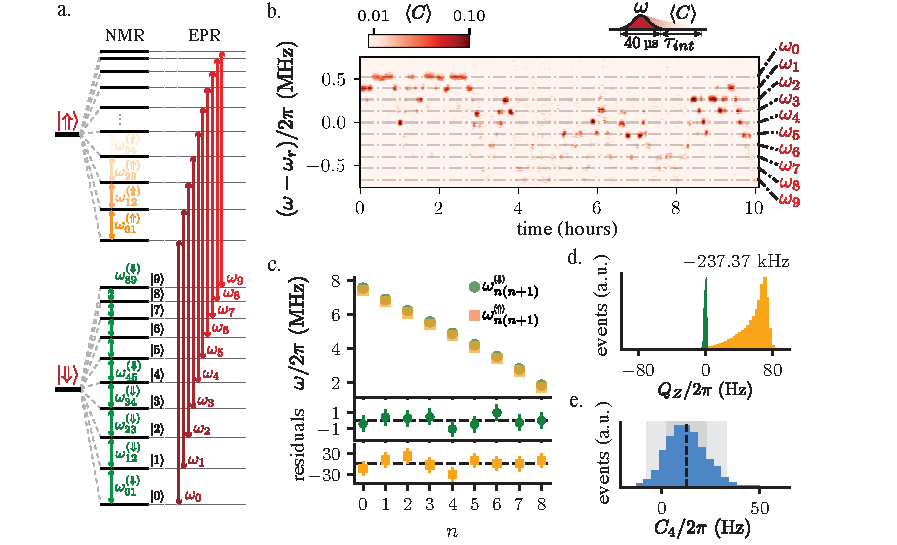
\includegraphics{chapter1/figures/ch3v1.pdf}
    \caption[Spectroscopie NMR de précision d'un spin nucléaire \Nb]{Spectroscopie NMR de précision d'un spin nucléaire \Nb.
    \textbf{a.} Spectre des niveaux d'énergie d'un spin \Er couplé à un spin nucléaire \Nb de spin $I=9/2$. Les dix transitions EPR permises sont indiquées en rouge. Les dix-huit transitions NMR permises sont mises en évidence en vert et en orange, selon l'état du spin \Er.
    \textbf{b.} Spectroscopie par comptage de photons d'un spin \Er unique couplé à un spin nucléaire \Nb en fonction du temps. La fréquence de détection du SMPD est accordée dynamiquement afin de correspondre à la fréquence $\omega$ de l'impulsion micro-onde appliquée. Les comptages moyennés sur l'ensemble $\langle C \rangle$ sont tracés en fonction de la fréquence de l'impulsion et du temps de mesure. Les dix fréquences EPR permises sont mises en évidence par une ligne grise pointillée. La séquence d'impulsions est indiquée en haut à droite.
    \textbf{c.} Spectre NMR et ajustement hamiltonien. \textit{(haut)} Les spectres NMR des transitions \Nb dans l'état fondamental (excité) du spin \Er sont tracés en vert (orange) en fonction de l'indice de transition $n$. \textit{(bas)} Résidus de l'ajustement hamiltonien. On obtient $\chi^2_\nu=1.2$, ce qui indique un ajustement satisfaisant. Les barres d'erreur correspondent à l'incertitude sur la fréquence et la ligne noire pointillée marque le zéro.
    \textbf{d.} Observation d'un quadrupôle dépendant du spin. Distribution a posteriori de la composante principale du tenseur quadrupolaire le long de l'axe $Z$ pour les ajustements de l'état fondamental et de l'état excité (vert et orange respectivement). Les distributions sont normalisées à la même hauteur pour une meilleure lisibilité.
    \textbf{e.} Intensité du couplage hexadécapolaire. Distributions a posteriori de la constante de couplage hexadécapolaire $C_4$. La ligne verticale indique la moyenne de la distribution et les zones ombrées les intervalles de confiance à $1$ et $2\,\sigma$.
    } 
    \labfig{ch3}
\end{figure*}

\section*{Spectroscopie de précision d'un spin 9/2}

\begin{marginfigure}
    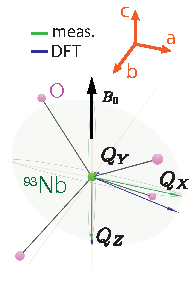
\includegraphics{chapter1/figures/ch3_extra.pdf}
    \caption[Reconstruction du tenseur quadrupolaire]{Représentation tridimensionnelle du tenseur quadrupolaire. Le spin nucléaire \Nb (vert) se situe au centre, entouré par les atomes d'oxygène voisins (rose). Les axes cristallins $a$, $b$ et $c$ sont indiqués par des lignes orange. Les axes principaux quadrupolaires mesurés $X$, $Y$ et $Z$ sont représentés par des flèches vertes, qui définissent les demi-axes d'un ellipsoïde, représenté en vert. Les vecteurs principaux obtenus par simulations DFT sont tracés en bleu foncé.}
    \labfig{ch3_extra}
\end{marginfigure}

Une autre application des méthodes développées au Chapitre \ref{ch:detection_and_control_of_individual_w} consiste à caractériser un atome inconnu situé à proximité d'un spin électronique. C'est l'objet du Chapitre \ref{ch:nb_nuclear_spin}, dans lequel nous caractérisons complètement une impureté inconnue de spin nucléaire 9/2 proche d'un spin \Er. Nous réalisons en outre une spectroscopie hyperfine de précision de cet atome \Nb et mettons en évidence des termes jusque-là inconnus dans l'Hamiltonien de spin.

La \reffig{ch3}a représente les vingt niveaux d'énergie du système couplé \Nb--\Er ainsi que l'ensemble des transitions EPR, de fréquences $\omega_n$, et des transitions NMR permises, séparées en deux familles selon l'état $m_S$ du spin \Er et de fréquences $\omega_{n,n+1}^{(m_S)}$. Nous caractérisons d'abord le système par spectroscopie EPR en mesurant des traces temporelles similaires à celles du Chapitre \ref{ch:detection_and_control_of_individual_w}. La \reffig{ch3}b montre les dix transitions EPR permises du spin électronique, régulièrement espacées, signature caractéristique d'un spin électronique couplé à un spin nucléaire $I=9/2$.

Nous utilisons les méthodes développées dans les chapitres précédents (lecture single-shot, DNP par effet solide et excitation Raman stimulée) pour mesurer le spectre NMR du spin \Nb. En comparant la fréquence de Larmor de l'impureté aux rapports gyromagnétiques de différents spins nucléaires, nous l'identifions comme étant un spin \Nb. Nous tirons parti de la longue cohérence du spin nucléaire pour mesurer son spectre hyperfin avec une résolution de l'ordre du hertz, présenté sur la \reffig{ch3}c en fonction de l'indice de transition. La grande séparation des niveaux indique que l'intensité de l'interaction quadrupolaire du spin nucléaire est du même ordre de grandeur que celle de l'interaction de Zeeman.

Nous ajustons le spectre NMR à un modèle hamiltonien dans les deux manifolds \Er avec une précision au hertz, comme le montrent les résidus de l'ajustement (présentés sur la \reffig{ch3}c). Nous utilisons ces résultats pour reconstruire le quadrupôle de \Nb et le comparer à des simulations DFT. La reconstruction du quadrupôle ainsi que le résultat DFT sont présentés sur la \reffig{ch3_extra}. Nous trouvons un accord quantitatif entre les deux, tant en amplitude qu'en orientation angulaire, ce qui indique une attribution correcte du site.

De plus, nous observons que l'intensité de l'interaction quadrupolaire diffère entre les deux manifolds, comme l'illustre la \reffig{ch3}d à travers la différence statistiquement significative entre les distributions a posteriori de la force de couplage quadrupolaire obtenues pour les deux ajustements. Nous attribuons cette différence à un nouveau type d'interaction entre spins électronique et nucléaire. Nous avançons que l'origine de cette interaction réside dans le couplage entre le dipôle électrique induit magnétiquement du spin \Er et l'interaction quadrupolaire nucléaire~\sidecite{bloembergen_linear_1961,mims_electric_1964}.

Enfin, nous parvenons à contraindre l'interaction hexadécapolaire avec des bornes environ un ordre de grandeur plus strictes que les mesures précédemment à l'état de l'art~\sidecite{liao_nuclear_1994}, comme le montre la \reffig{ch3}e.